\documentclass{standalone}
\usepackage{tikz}
\usetikzlibrary{patterns, positioning}
\usetikzlibrary{shapes.misc}
\usepackage[outline]{contour}
\contourlength{1.5pt} 


\begin{document}
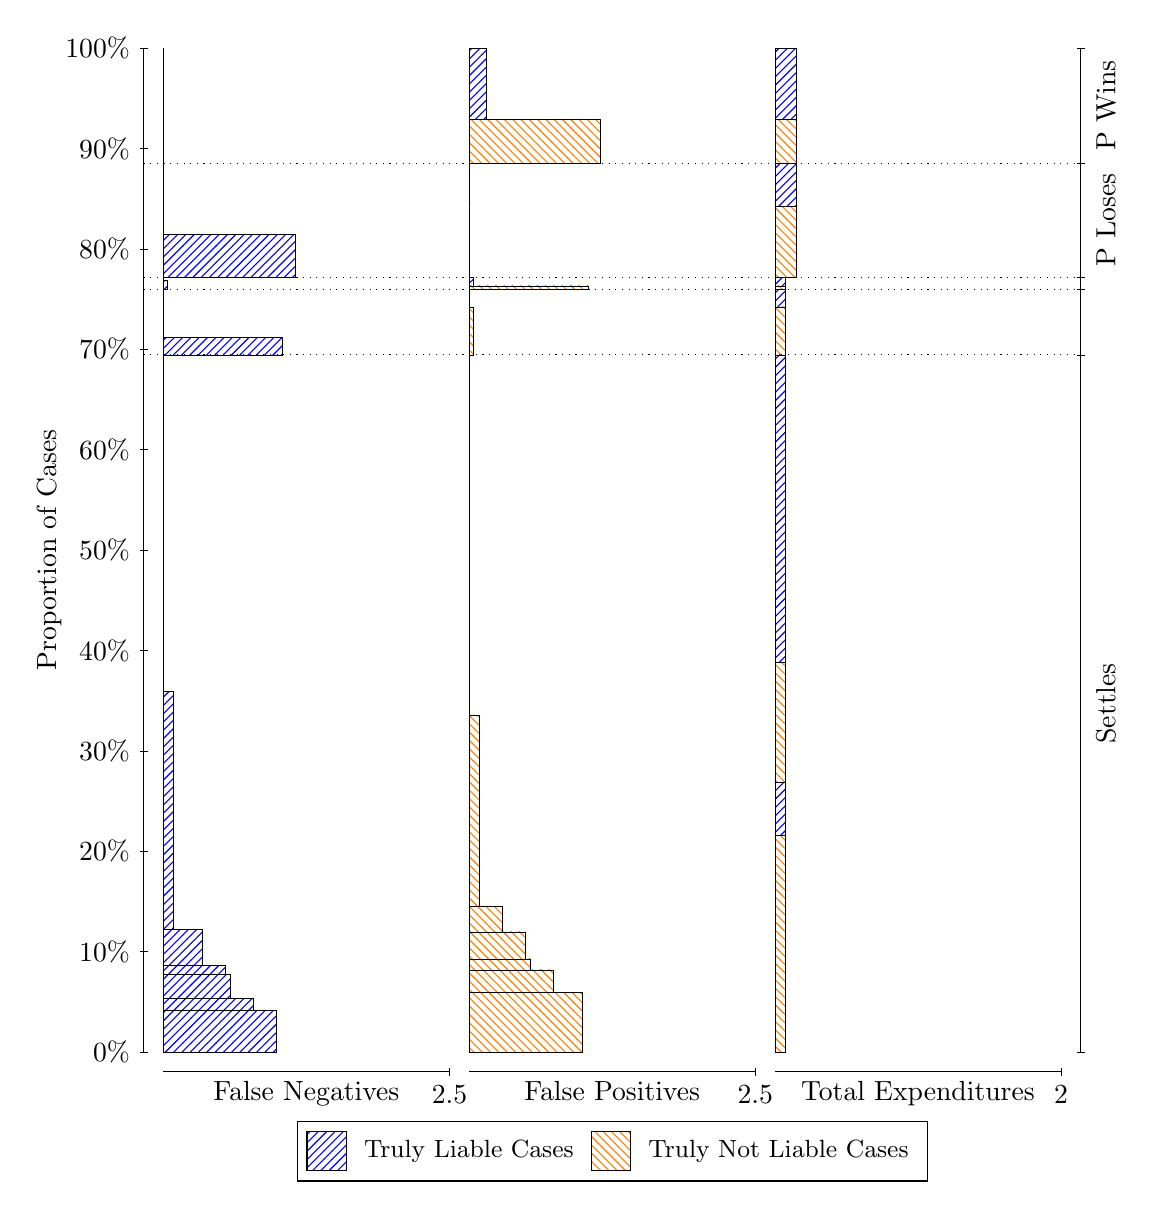
\begin{tikzpicture}
\draw[black, very thin] (1.5,1.75) -- (1.5,14.5);
\node[rotate=90, text=black, anchor=center] at (0.3, 8.125) {Proportion of Cases};
\draw[black, very thin] (1.45,1.75) -- (1.55,1.75);
\node[text=black, anchor=east] at (1.45, 1.75) {0\%};
\draw[black, very thin] (1.45,3.025) -- (1.55,3.025);
\node[text=black, anchor=east] at (1.45, 3.025) {10\%};
\draw[black, very thin] (1.45,4.3) -- (1.55,4.3);
\node[text=black, anchor=east] at (1.45, 4.3) {20\%};
\draw[black, very thin] (1.45,5.575) -- (1.55,5.575);
\node[text=black, anchor=east] at (1.45, 5.575) {30\%};
\draw[black, very thin] (1.45,6.85) -- (1.55,6.85);
\node[text=black, anchor=east] at (1.45, 6.85) {40\%};
\draw[black, very thin] (1.45,8.125) -- (1.55,8.125);
\node[text=black, anchor=east] at (1.45, 8.125) {50\%};
\draw[black, very thin] (1.45,9.4) -- (1.55,9.4);
\node[text=black, anchor=east] at (1.45, 9.4) {60\%};
\draw[black, very thin] (1.45,10.675) -- (1.55,10.675);
\node[text=black, anchor=east] at (1.45, 10.675) {70\%};
\draw[black, very thin] (1.45,11.95) -- (1.55,11.95);
\node[text=black, anchor=east] at (1.45, 11.95) {80\%};
\draw[black, very thin] (1.45,13.225) -- (1.55,13.225);
\node[text=black, anchor=east] at (1.45, 13.225) {90\%};
\draw[black, very thin] (1.45,14.5) -- (1.55,14.5);
\node[text=black, anchor=east] at (1.45, 14.5) {100\%};

\draw[black, very thin] (13.4,1.75) -- (13.4,14.5);
\draw[black, very thin] (13.35,1.75) -- (13.45,1.75);
\node[anchor=west] at (13.35, 1.75) {};
\draw[black, very thin] (13.35,10.604) -- (13.45,10.604);
\node[anchor=west] at (13.35, 10.604) {};
\draw[black, very thin] (13.35,11.438) -- (13.45,11.438);
\node[anchor=west] at (13.35, 11.438) {};
\draw[black, very thin] (13.35,11.586) -- (13.45,11.586);
\node[anchor=west] at (13.35, 11.586) {};
\draw[black, very thin] (13.35,13.038) -- (13.45,13.038);
\node[anchor=west] at (13.35, 13.038) {};
\draw[black, very thin] (13.35,14.5) -- (13.45,14.5);
\node[anchor=west] at (13.35, 14.5) {};

\draw[black, very thin, pattern color=blue, pattern=north east lines] (1.75,1.75) rectangle (3.1852,2.2759);
\draw[black, very thin, pattern color=blue, pattern=north east lines] (1.75,2.2759) rectangle (2.8945,2.4316);
\draw[black, very thin, pattern color=blue, pattern=north east lines] (1.75,2.4316) rectangle (2.6038,2.7331);
\draw[black, very thin, pattern color=blue, pattern=north east lines] (1.75,2.7331) rectangle (2.5312,2.8496);
\draw[black, very thin, pattern color=blue, pattern=north east lines] (1.75,2.8496) rectangle (2.2405,3.3025);
\draw[black, very thin, pattern color=blue, pattern=north east lines] (1.75,3.3025) rectangle (1.8772,6.3318);
\draw[black, very thin, pattern color=orange, pattern=north west lines] (1.75,6.3318) rectangle (1.75,10.604);
\draw[black, very thin, pattern color=blue, pattern=north east lines] (1.75,10.604) rectangle (3.2578,10.83);
\draw[black, very thin, pattern color=orange, pattern=north west lines] (1.75,10.83) rectangle (1.75,11.438);
\draw[black, very thin, pattern color=blue, pattern=north east lines] (1.75,11.438) rectangle (1.8045,11.545);
\draw[black, very thin, pattern color=orange, pattern=north west lines] (1.75,11.545) rectangle (1.75,11.586);
\draw[black, very thin, pattern color=blue, pattern=north east lines] (1.75,11.586) rectangle (3.4213,12.136);
\draw[black, very thin, pattern color=orange, pattern=north west lines] (1.75,12.136) rectangle (1.75,13.038);
\draw[black, very thin, pattern color=orange, pattern=north west lines] (1.75,13.038) rectangle (1.75,13.589);
\draw[black, very thin, pattern color=blue, pattern=north east lines] (1.75,13.589) rectangle (1.75,14.5);
\draw[black, very thin, pattern color=orange, pattern=north west lines] (5.6333,1.75) rectangle (7.0685,2.5104);
\draw[black, very thin, pattern color=orange, pattern=north west lines] (5.6333,2.5104) rectangle (6.7052,2.7936);
\draw[black, very thin, pattern color=orange, pattern=north west lines] (5.6333,2.7936) rectangle (6.4145,2.932);
\draw[black, very thin, pattern color=orange, pattern=north west lines] (5.6333,2.932) rectangle (6.3418,3.2746);
\draw[black, very thin, pattern color=orange, pattern=north west lines] (5.6333,3.2746) rectangle (6.0512,3.6021);
\draw[black, very thin, pattern color=orange, pattern=north west lines] (5.6333,3.6021) rectangle (5.7605,6.0226);
\draw[black, very thin, pattern color=blue, pattern=north east lines] (5.6333,6.0226) rectangle (5.6333,10.604);
\draw[black, very thin, pattern color=orange, pattern=north west lines] (5.6333,10.604) rectangle (5.6878,11.212);
\draw[black, very thin, pattern color=blue, pattern=north east lines] (5.6333,11.212) rectangle (5.6333,11.438);
\draw[black, very thin, pattern color=orange, pattern=north west lines] (5.6333,11.438) rectangle (7.1412,11.479);
\draw[black, very thin, pattern color=blue, pattern=north east lines] (5.6333,11.479) rectangle (5.6878,11.586);
\draw[black, very thin, pattern color=orange, pattern=north west lines] (5.6333,11.586) rectangle (5.6333,12.489);
\draw[black, very thin, pattern color=blue, pattern=north east lines] (5.6333,12.489) rectangle (5.6333,13.038);
\draw[black, very thin, pattern color=orange, pattern=north west lines] (5.6333,13.038) rectangle (7.3047,13.589);
\draw[black, very thin, pattern color=blue, pattern=north east lines] (5.6333,13.589) rectangle (5.8513,14.5);
\draw[black, very thin, pattern color=orange, pattern=north west lines] (9.5167,1.75) rectangle (9.6529,4.498);
\draw[black, very thin, pattern color=blue, pattern=north east lines] (9.5167,4.498) rectangle (9.6529,5.1795);
\draw[black, very thin, pattern color=orange, pattern=north west lines] (9.5167,5.1795) rectangle (9.6529,6.7042);
\draw[black, very thin, pattern color=blue, pattern=north east lines] (9.5167,6.7042) rectangle (9.6529,10.604);
\draw[black, very thin, pattern color=orange, pattern=north west lines] (9.5167,10.604) rectangle (9.6529,11.212);
\draw[black, very thin, pattern color=blue, pattern=north east lines] (9.5167,11.212) rectangle (9.6529,11.438);
\draw[black, very thin, pattern color=orange, pattern=north west lines] (9.5167,11.438) rectangle (9.6529,11.479);
\draw[black, very thin, pattern color=blue, pattern=north east lines] (9.5167,11.479) rectangle (9.6529,11.586);
\draw[black, very thin, pattern color=orange, pattern=north west lines] (9.5167,11.586) rectangle (9.7892,12.489);
\draw[black, very thin, pattern color=blue, pattern=north east lines] (9.5167,12.489) rectangle (9.7892,13.038);
\draw[black, very thin, pattern color=orange, pattern=north west lines] (9.5167,13.038) rectangle (9.7892,13.589);
\draw[black, very thin, pattern color=blue, pattern=north east lines] (9.5167,13.589) rectangle (9.7892,14.5);
\draw[black, dotted] (1.5,10.604) -- (13.4,10.604);
\draw[black, dotted] (1.5,11.438) -- (13.4,11.438);
\draw[black, dotted] (1.5,11.586) -- (13.4,11.586);
\draw[black, dotted] (1.5,13.038) -- (13.4,13.038);
\draw[black, very thin] (1.75,1.5) -- (5.3833,1.5);
\node[text=black, anchor=north] at (3.5667, 1.5) {False Negatives};
\draw[black, very thin] (5.3833,1.45) -- (5.3833,1.55);
\node[text=black, anchor=north] at (5.3833, 1.45) {2.5};

\draw[black, very thin] (5.6333,1.5) -- (9.2667,1.5);
\node[text=black, anchor=north] at (7.45, 1.5) {False Positives};
\draw[black, very thin] (9.2667,1.45) -- (9.2667,1.55);
\node[text=black, anchor=north] at (9.2667, 1.45) {2.5};

\draw[black, very thin] (9.5167,1.5) -- (13.15,1.5);
\node[text=black, anchor=north] at (11.333, 1.5) {Total Expenditures};
\draw[black, very thin] (13.15,1.45) -- (13.15,1.55);
\node[text=black, anchor=north] at (13.15, 1.45) {2};

\node[text=black, centered, rotate=90] at (13.72, 6.1772) {\contour{white}{Settles}};


\node[text=black, centered, rotate=90] at (13.72, 12.312) {\contour{white}{P Loses}};
\node[text=black, centered, rotate=90] at (13.72, 13.769) {\contour{white}{P Wins}};

\draw (7.449999999999999,1.5) node[draw=none] (baseCoordinate) {};
\begin{scope}[align=center]
        \matrix[scale=0.5, draw=black, below=0.5cm of baseCoordinate, nodes={draw}, column sep=0.1cm]{
            \node[rectangle, draw, minimum width=0.5cm, minimum height=0.5cm, pattern color=blue, pattern=north east lines] {}; &
            \node[draw=none, font=\small, text=black] (B) {Truly Liable Cases}; &
            \node[rectangle, draw, minimum width=0.5cm, minimum height=0.5cm, pattern color=orange, pattern=north west lines] {}; &
            \node[draw=none, font=\small, text=black] (B) {Truly Not Liable Cases}; \\
            };
\end{scope}

\end{tikzpicture}
\end{document}